\chapter{Results and Discussion}

The metric used here \(RMS_{2D}\) has been detailed in Chapter 3. These results were obtained from the implementation in Chapter 4.

\section{Quantitative Results}

\begin{table}[h]
\begin{tabular}{|l|l|l|l|l|}
\hline
RNN Size&Epochs& Input sequence length & Output Sequence Length \\
\hline
400       & 50      & 360      & 2   \\
\hline
400        & 50      & 204      & 2   \\
\hline
400     & 50      & 204          & 2\\
\hline
400    & 50      & 207          & 30\\
\hline
400  & 50      & 14k          & 10\\
\hline
400     & 50 & 1068 pedestrian, 464 cyclist trajectories & 20\\
\hline
\end{tabular}
\caption{Results}
\label{table:results}

\end{table}
Across all iterations, the loss was not reducing significantly beyond 25 epochs and hence the number of epochs were capped at 30 epochs. One epoch is one pass through the entire dataset. Batch gradient descent was used 

Keeping all other parameters constant, we see that the loss is higher when the output prediction window is high. This could be because predictions made on 
\section{Qualitative Results}



\begin{figure}[ht]
    \centering
    \subfigure[Predicted trajectory with low accuracy]
    {
        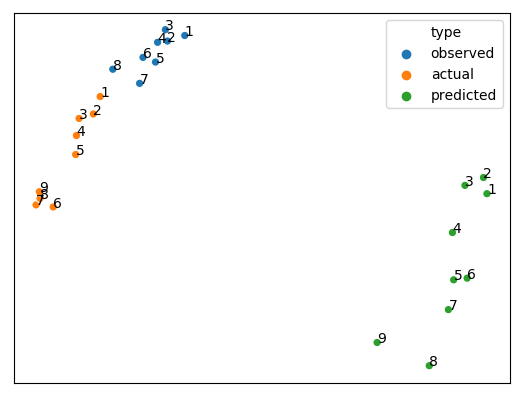
\includegraphics[width=0.43\linewidth]{Figures/Traj_low.png}
        \label{fig:Qual_analysis_a}
    }
    \qquad
    \subfigure[Predicted trajectory with high accuracy]
    {
        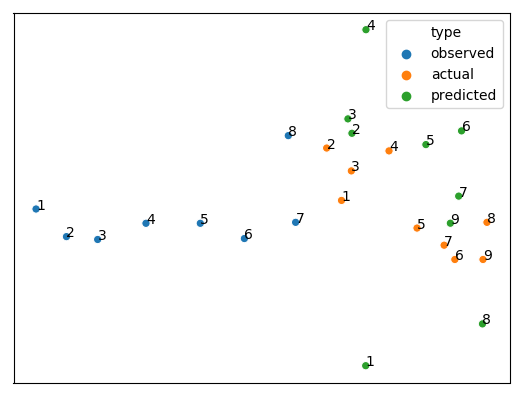
\includegraphics[width=0.43\linewidth]{Figures/Traj_high.png}
        \label{fig:Qual_analysis_b}
    }
    \caption
    {Qualitative analysis of 2 cases
    }
    \label{fig:Qual_analysis}
\end{figure}

yes, \ref{fig:Qual_analysis_a}

\section{Discussion}

What we did not do well. 
What could have done better. 

About modelling uncertainty and thus getting better results

An thorough exhaustive search for hyper-parameters using Grid search could have been used in order to conduct thorough hyper-parameter search. 
More efficient methods to deal with data could be employed
Other architectures could have been tried out.

